%%%%%%%%%%%%%%%%%%%%%%%%%%%%%%%%%%%%%%%%%
% Short Sectioned Assignment
% LaTeX Template
% Version 1.0 (5/5/12)
%
% This template has been downloaded from:
% http://www.LaTeXTemplates.com
%
% Original author:
% Frits Wenneker (http://www.howtotex.com)
%
% License:
% CC BY-NC-SA 3.0 (http://creativecommons.org/licenses/by-nc-sa/3.0/)
%
%%%%%%%%%%%%%%%%%%%%%%%%%%%%%%%%%%%%%%%%%

%----------------------------------------------------------------------------------------
%	PACKAGES AND OTHER DOCUMENT CONFIGURATIONS
%----------------------------------------------------------------------------------------

\documentclass[paper=a4, fontsize=12pt]{scrartcl} % A4 paper and 11pt font size
\usepackage{multirow}
\usepackage[T1]{fontenc} % Use 8-bit encoding that has 256 glyphs
\usepackage{fourier} % Use the Adobe Utopia font for the document - comment this line to return to the LaTeX default
\usepackage[english]{babel} % English language/hyphenation
\usepackage{amsmath,amsfonts,amsthm} % Math packages
\usepackage{booktabs}
\usepackage{sectsty} % Allows customizing section commands
\allsectionsfont{\centering \normalfont\scshape} % Make all sections centered, the default font and small caps
\usepackage{rotating}
\usepackage{graphicx}

\usepackage[a4paper,lmargin=2.5 cm,rmargin=2 cm,tmargin=2 cm,bmargin=2 cm]{geometry}

\usepackage{fancyhdr} % Custom headers and footers
\pagestyle{fancyplain} % Makes all pages in the document conform to the custom headers and footers
\fancyhead{} % No page header - if you want one, create it in the same way as the footers below
\fancyfoot[L]{} % Empty left footer
\fancyfoot[C]{} % Empty center footer
\fancyfoot[C]{\thepage} % Page numbering for right footer
\renewcommand{\headrulewidth}{0pt} % Remove header underlines
\renewcommand{\footrulewidth}{0pt} % Remove footer underlines
\setlength{\headheight}{13.6pt} % Customize the height of the header

\usepackage{chngcntr}
%\numberwithin{equation}{section} % Number equations within sections (i.e. 1.1, 1.2, 2.1, 2.2 instead of 1, 2, 3, 4)
%\numberwithin{figure}{section} % Number figures within sections (i.e. 1.1, 1.2, 2.1, 2.2 instead of 1, 2, 3, 4)
%\counterwithout{figure}{section}
%\numberwithin{table}{section} % Number tables within sections (i.e. 1.1, 1.2, 2.1, 2.2 instead of 1, 2, 3, 4)

%\setlength\parindent{0pt} % Removes all indentation from paragraphs - comment this line for an assignment with lots of text
\setlength\parindent{24pt}

\usepackage{amsmath}
\usepackage{float} % To firce the location of figure
\usepackage{subfigure} %For side-by-side figures
\usepackage{lettrine}
%\usepackage{lipsum}
\usepackage{epstopdf} %To read *.eps Files
\usepackage{listings} % To include source codes in LATEX document
\usepackage{mathrsfs} % To include script fonts. use \mathscr{}
\usepackage{courier} % To write in courier fornt
\usepackage{mathtools} % For mat symbols
\usepackage{xfrac} % For \sfrac{}{}
\usepackage{listings}
%----------------------------------------------------------------------------------------
%	TITLE SECTION
%----------------------------------------------------------------------------------------

\newcommand{\horrule}[1]{\rule{\linewidth}{#1}} % Create horizontal rule command with 1 argument of height

\title{	
\normalfont \normalsize 
\textsc{Wright State University\\ Department of Mechanical and Materials Engineering} \\ [25pt] % Your university, school and/or department name(s)
\horrule{0.5pt} \\[0.4cm] % Thin top horizontal rule
\huge Vibration Testing and Health Monitoring \\ % The assignment title
\Large Final Exam
\horrule{2pt} \\[0.5cm] % Thick bottom horizontal rule
}

\author{Admir Makas} % Your name

\date{\normalsize April 28, 2016} % Today's date or a custom date

\begin{document}

\maketitle % Print the title

%----------------------------------------------------------------------------------------
%	Introduction
%----------------------------------------------------------------------------------------
\section*{Write Up}
Three FRF's for $H_{11}$, $H_{12}$, and $H_{13}$ were provided. The goal is to perform system identification using the Ho-Kalman method. Markov parameters were constructed from the provided data using two methods. The first method can be seen in Figure \ref{fig:M1}. Each of the Markov parameters were constructed in this fashion for a total of 803.
%
\begin{figure}[H]
	\centering
	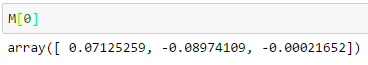
\includegraphics[height = 2.0cm]{M1.png}
	\caption{Markov parameter definition for Option 1}
	\label{fig:M1}
\end{figure}
%
The second method for constructing the Markov parameters can be seen in Figure \ref{fig:M2}. The main idea here is that the Markov matrices are symmetric. Therefore, values of the matrix 12=21 and 13=31. Values for which Markov parameters do not exist are set to zero
%
\begin{figure}[H]
	\centering
	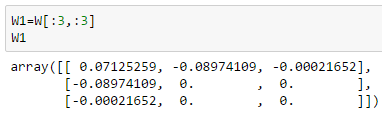
\includegraphics[height = 3.5cm]{M2.png}
	\caption{Markov parameter definition for Option 2}
	\label{fig:M2}
\end{figure}
%
Using the above definitions $H(0)$, and $H(1)$ were constructed. For a full detail of the math performed please see the IPython notebook files. The next figure shows the significant values from the Sigma matrix. For option 1, there are 6 significant values. For option 2 there are 12. Figure \ref{fig:SigmaPlotBoth} shows a plot for Sigma values in order to illustrate the decreasing trend.
%
\begin{figure}[H]
	\centering
	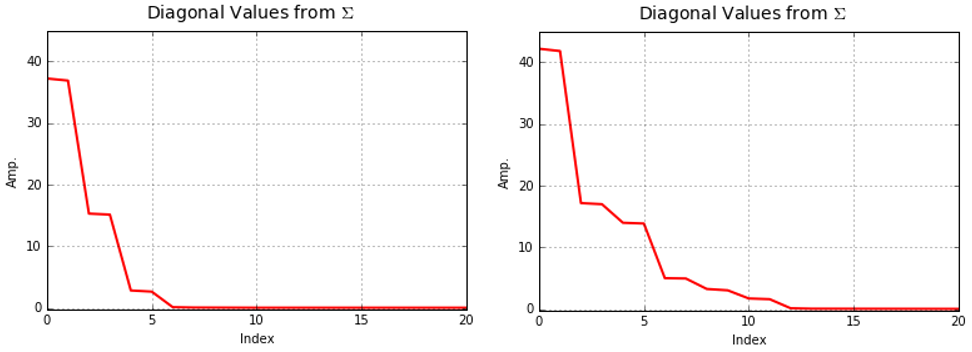
\includegraphics[height = 5.0cm]{SigmaPlotBoth.png}
	\caption{Plots showing Sigma values.}
	\label{fig:SigmaPlotBoth}
\end{figure}
%
Table \ref{tab:NatFreq} shows the natural frequency estimations for options 1 and 2 and compares them to experimental data. Both methods estimated same values for natural frequencies.
%
\begin{table}[H]
  \centering
  \caption{System natural frequencies}
    \begin{tabular}{rccc}
    \toprule
          & \multicolumn{3}{c}{\textbf{Natural Frequencies (Hz)}} \\
    \midrule
    \multicolumn{1}{c}{} & \textbf{Option 1} & \textbf{Option 2} & \textbf{Exp. Data} \\
    \multicolumn{1}{c}{$\omega_1$} & 0.1016 & 0.1015 & 0.103 \\
    \multicolumn{1}{c}{$\omega_2$} & 0.1937 & 0.1937 & 0.196 \\
    \multicolumn{1}{c}{$\omega_3$} & 0.3207 & 0.3207 & 0.325 \\
    \bottomrule
    \end{tabular}%
  \label{tab:NatFreq}%
\end{table}%
%
%
Since natural frequencies are same for options 1 and 2 it follows that estimations of the damping ratios $\zeta$ will also be the same. Their values are listed in Table \ref{tab:DampRat}.
%
\begin{table}[H]
  \centering
  \caption{System damping ratios}
    \begin{tabular}{rcc}
    \toprule
          & \multicolumn{2}{c}{\textbf{Damping Ratios}} \\
    \midrule
    \multicolumn{1}{c}{} & \textbf{Option 1} & \textbf{Option 2} \\
    \multicolumn{1}{c}{$\zeta_1$} & 0.00274 & 0.00274 \\
    \multicolumn{1}{c}{$\zeta_2$} & 0.00327 & 0.00327 \\
    \multicolumn{1}{c}{$\zeta_3$} & 0.00787 & 0.00789 \\
    \bottomrule
    \end{tabular}%
  \label{tab:DampRat}%
\end{table}%
%
%
Based on the information gained from the Sigma plots, Option 1 will have a state space comprised of 6 states and option 2 will have 12 states. The state space models defined for options 1 and 2 are used to reconstruct the FRF's, which are compared with respect to the original data. Starting first with $H_{11}$ estimate in Figure \ref{fig:H11EstBoth}.
%
\begin{figure}[H]
	\centering
	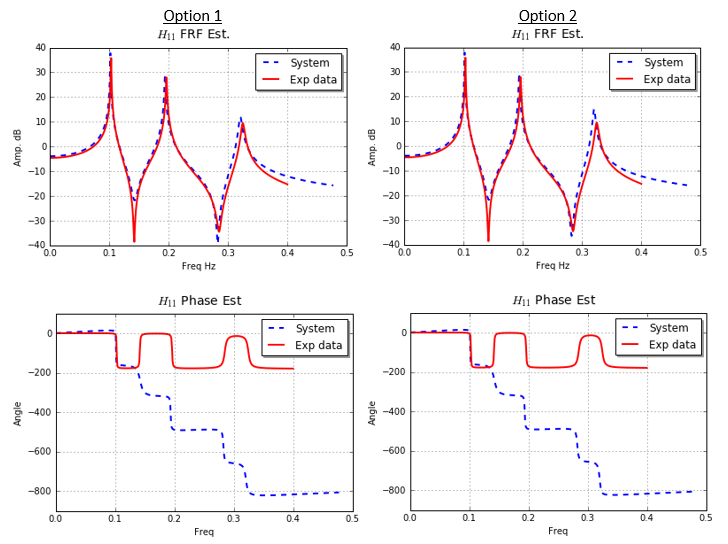
\includegraphics[height = 12.5cm]{H11EstBoth.png}
	\caption{FRF 11 estimate compared with original data.}
	\label{fig:H11EstBoth}
\end{figure}
%
For the FRF 11 estimate, both option 1 and 2 do a good job of obtaining the correct amplitude plots. Despite this fact, the phase diagrams are registering a -90 degree phase shift at the zero locations. Not sure yet as to why this is happening.
%
\\
\\
%
The next Figure shows the FRF 12 estimate. For this signal, option 2 shows a considerable improvement in both the amplitude plot and phase diagram. For one, option 2 amplitude plot estimates the peaks more accurately. Second, it also pick up the zero, which is missing in the option 1 amplitude plot. As a result, the phase diagram is markedly improved for option 2 vs. option 1 fit.
%
\begin{figure}[H]
	\centering
	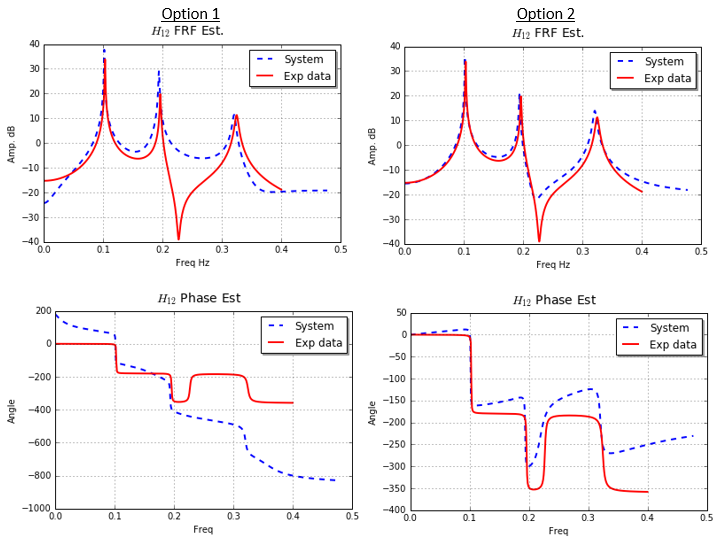
\includegraphics[height = 12.5cm]{H12EstBoth.png}
	\caption{FRF 12 estimate compared with original data.}
	\label{fig:H12EstBoth}
\end{figure}
%
Finally, Figure \ref{fig:H13EstBoth} shows the FRF 13 estimate. In similar fashion, option 2 estimate is better at overall fit of the amplitude data. It also estimates the peaks better. The better amplitude estimate is also seen in the phase plot estimations as well.
%
\begin{figure}[H]
	\centering
	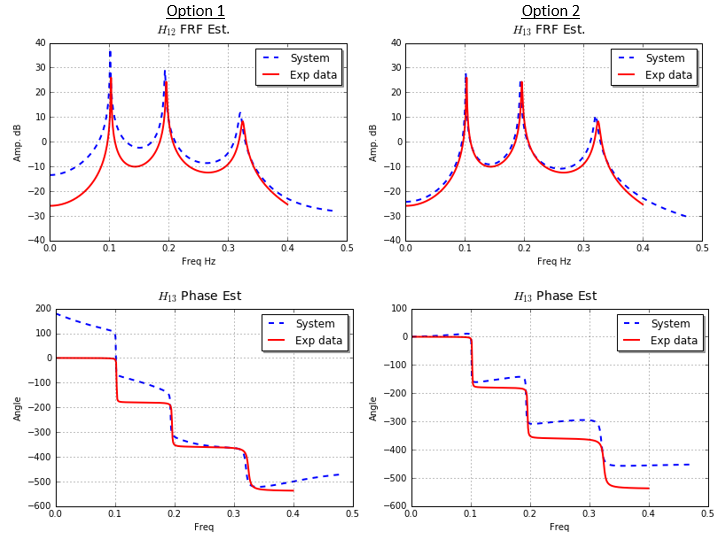
\includegraphics[height = 12.5cm]{H13EstBoth.png}
	\caption{FRF 12 estimate compared with original data.}
	\label{fig:H13EstBoth}
\end{figure}
%
In closing, it is not sure why option 2 performs a better estimations. Technically the provided system has 6 states but option 2 works by using 12 states instead. As such, there should be a way to obtain a 6 degree of freedom state space matrix A from the 12 degree state space model. This will be investigated further in the future.



\end{document}